\documentclass[11pt,twoside,a4paper]{article}

\usepackage[pdftex]{graphicx}
\usepackage[pdftex]{hyperref}

\begin{document}

\title{SAMM: Simple Accelerator Modelling in Matlab}
\author{A.\,Wolski}
\date{Version 2.5: April 27, 2013}

\maketitle

\begin{abstract}
SAMM is a set of Matlab routines for modelling beam dynamics in particle
accelerators.  This note explains the installation, general features and
overall structure. The use of SAMM is discussed, and illustrated with some
simple examples.
\end{abstract}

\newpage

\tableofcontents

\newpage

\section{Getting started}
In this section, we give a brief explanation of the purpose and capabilities
of SAMM, describe how to install it, and discuss some simple examples.

\subsection{Introduction to SAMM}
SAMM is a set of Matlab \cite{cite:matlab} routines for modelling beam dynamics
in high energy particle accelerators.  To develop an application, the user writes
Matlab scripts that call classes and functions defined in SAMM.  In other words,
SAMM consists of a library from which an accelerator simulation may be developed.
The intentions behind SAMM are: for the
physics to be as accurate as possible; for the code to be as short and simple as
possible; and for the structure of the code to reflect as closely as possible the
structure of a real accelerator.  It is also intended that the code be structured
to make it as easy as possible to extend its capabilities: that is, it should be
straightforward for the user to add new beamline
components, dynamical effects, and analysis procedures, as required.

Since simplicity and brevity are prioritised over performance, SAMM is unlikely to be
the best code for large-scale simulations of complex accelerator systems.
However, some effort has been made to make the code reasonably efficient, so for
relatively simple systems, the speed of computation should be acceptable.

To achieve a logical and clear structure in SAMM, extensive use is made of
object-oriented programming features in Matlab.  Users are recommended to familiarise
themselves with the section on ``Object-Oriented Programming'' in the Matlab
documentation \cite{cite:matlabdoc}, before working with SAMM.

The latest version of SAMM has been tested with Matlab Release 2012a.
Compatibility with earlier versions of Matlab is not guaranteed.

\subsection{Installation}
Installation of SAMM is accomplished in three steps.
\begin{enumerate}
\item Download the archive SAMM2.5.zip from:
\begin{quote}
\texttt{\small http://pcwww.liv.ac.uk/$\sim$awolski/main\_links\_computercodes.htm}
\end{quote}
\item Extract the contents of the archive to any convenient
location on your hard drive.
\item Launch Matlab, and from the ``File... Set Path...'' menu option, add the
main SAMM directory and all subdirectories to the Matlab path.  It is recommended
that the path be saved for future sessions.
\end{enumerate}

\subsection{Structure}
The overall structure of SAMM is best understood through the directory
structure.  There are three important subdirectories within the main SAMM
directory:
\paragraph{SAMMlab} contains class definitions for a beam, an accelerator
beam line, some useful physical constants, physical units and utilities.
\paragraph{Particles} contains class definitions that specify the properties of particles that can constitute a beam.
\paragraph{Components} contains class definition for accelerator components.
An accelerator beam line consists of a sequence of components.
\paragraph{Physics} contains a set of functions for performing analysis of
the beam dynamics in a beam line.
\paragraph{}

Additionally, there are subdirectories for documentation and examples.  Also within
the main directory is a file SAMM.m; the only functionality of this file is to
provide text in response to the user command:
\begin{quote}
\texttt{>> help SAMM}
\end{quote}

\subsection{A simple example: tracking a beam through a beam line\label{sec:simpleexample}}
In this section, we present a simple example that shows how to set up a beam line,
how to define a beam, and how to track the beam through the beam line.

\subsubsection{Defining the components in the beam line}
The first step is to define the components that comprise the beam line.
For example, the commands:
\begin{quote}
\texttt{>> drift1 = Drift; \\
>> drift1.length = 1.5;}
\end{quote}
define a drift of length 1.5\,m; and the commands:
\begin{quote}
\texttt{>> quad1 = Quadrupole; \\
>> quad1.length = 0.3; \\
>> quad1.gradient = 0.8;}
\end{quote}
define a quadrupole magnet of length 0.3\,m, and field gradient 0.8\,T/m.

\subsubsection{Defining the beam line}
The second step is to define the beam line as a sequence of components.
For example, the commands:
\begin{quote}
\texttt{>> beamline1 = Beamline; \\
>> beamline1.componentlist = \{quad1,drift1\};}
\end{quote}
define a beam line consisting of the quadrupole followed by the drift space
previously defined.  More information on constructing a beam line is given
below, in Section~\ref{sec:settingupabeamline}

\subsubsection{Defining the beam}
To track particles through the beam line, we need to define a beam.  A beam
consists of a set of particles of specified type.  All particles in the beam
are of the same type.  For example, a beam of positrons can be defined with
the assignment:
\begin{quote}
\texttt{>> beam1 = Beam(Positron);}
\end{quote}
Note that
\texttt{Positron} is a class name.  Since the particle properties (mass, charge,
etc.) are defined as \texttt{Constant} within the class, it is not necessary
to define an object of that class: the class itself can be passed as a parameter
to the beam definition.

Each particle in the beam has coordinates and momenta specified with respect
to a local coordinate system (see Section~\ref{sec:modellingabeam}).  The energy
of each particle is expressed as a deviation from some nominal \emph{reference
energy}, $E_0$.  The reference energy should be specified after defining the beam;
for example, following the above definition of a beam of positrons, the reference
energy of the beam can be specified by:
\begin{quote}
\texttt{>> beam1.energy = 1.20*PhysicalUnits.GeV;}
\end{quote}
Note that the value
of the energy specified in the beam definition must be given in joules: the class
\texttt{PhysicalUnits} in SAMM defines a conversion factor \texttt{GeV} that
converts a quantity given in GeV to units of joules.

Associated with the reference energy are a \emph{reference momentum} $P_0$,
defined so that:
\[
E_0^2 = P_0^2 c^2 + m^2 c^4,
\]
where $m$ is the rest mass of each particle in the beam; and a \emph{beam
rigidity} $B\rho$, defined by:
\[
B\rho = \frac{P_0}{q},
\]
where $q$ is the electric charge of each particle in the beam.  The reference
momentum and beam rigidity are explained further in Section~\ref{sec:modellingabeam}.
But for now, note that for a given particle species, defining any one of these quantities
(reference energy, reference momentum, beam rigidity) allows the other two to be
calculated.  In SAMM, the user can specify any of these quantities for a beam; and SAMM
will then return the value (when asked) for any of them.  For example:
\begin{quote}
\texttt{>> beam1.energy = 1.20*PhysicalUnits.GeV; \\
>> beam1.rigidity \\
ans = 4.0028 \\
>> beam1.momentum \\
ans = 6.4131e-019
}
\end{quote}
The beam rigidity has units of T\,m (tesla metres), and the momentum
has units of kg\,m\,s$^{-1}$.

Note that the momenta of particles in the beam are defined with respect to
the reference momentum (see Section~\ref{sec:modellingabeam}).  If you
redefine the reference energy, reference momentum, or beam rigidity of a 
beam, then if the beam contains any particles, the relative momenta of these
particles will be scaled, so that the absolute momenta remain the same.

The coordinates and momenta of the particles in the beam are contained in a
$6\times N$ matrix, where $N$ is the number of particles in the beam.  Each
column of the matrix corresponds to a different particle; each row corresponds
to a different \emph{dynamical variable}.  The dynamical variables describe
the position and momentum of a particle: more information is given in
Section~\ref{sec:modellingabeam}.  As an example, the commands:
\begin{quote}
\texttt{>> ptcle1 = [0.001,0,0,0,0,0]$^\prime$; \\
>> ptcle2 = [0,0,0.001,0,0,0]$^\prime$;}
\end{quote}
define two particles: the first with $x$ coordinate 0.001\,m, and the second
with $y$ coordinate 0.001\,m.  Particles are added to the beam as follows:
\begin{quote}
\texttt{>> beam1.particles = [ptcle1 ptcle2];}
\end{quote}

Particle spins can be specified in a similar way to the dynamical variables.
The spin of a particle is defined in terms of the orientation of its spin axis with
respect to the reference trajectory in the instantaneous rest frame of the
particle.  For example:
\begin{quote}
\texttt{>> beam1.spins = s;}
\end{quote}
would specify the orientation of the spin of each particle in \texttt{beam1}.
\texttt{s} must be a $2\times N$ matrix, where $N$ is the number of particles
in the beam.  The first row of \texttt{s} gives the polar angle $\theta$ (the
angle of the spin axis of each particle, with respect to the reference trajectory);
the second row of \texttt{s} gives the azimuthal angle $\phi$ (the angle of the
projection of the spin axis on the $x-y$ plane, with respect to the $x$ axis).
For more information, see Section~\ref{subsec:spin}.


\subsubsection{Tracking the beam through the beam line}
The command:
\begin{quote}
\texttt{>> beam2 = beamline1.Track([1 2],beam1);}
\end{quote}
will track the beam previously defined through the first two components in the
beam line \texttt{beamline1}.  For the beam line defined in the example in step 3 above,
there are only two component: a quadrupole, followed by a drift.  In this case,
the $6\times 2$ matrix \texttt{beam2.particles} will be:
\[
\texttt{beam2} = \left[ \begin{array}{cc}
 0.00090135149           & 0 \\
-0.00005977817	         & 0 \\
 0	                     & 0.0010992147 \\
 0                       & 0.000060138318 \\
-2.8592354\times 10^{-9} & 	-2.8928612\times 10^{-8} \\
 0                       & 0
\end{array}
\right]
\]


\subsection{More about beam lines\label{sec:settingupabeamline}}
As explained in Section~\ref{sec:simpleexample}, a beam line is defined as
a sequence of components.  The components must first be individually
defined, then added to the beam line.  An important feature of SAMM is
that an individual element can be added multiple times to a beam line.
Changing the parameters of the component will then change the parameters
for every instance of that component in the beam line.  For example,
consider the following beam line definition:
\begin{quote}
\texttt{>> drift1 = Drift; \\
>> drift1.length = 0.5; \\
>> quad1 = Quadrupole; \\
>> quad1.length = 0.25; \\
>> quad1.gradient = -0.3; \\
>> beamline1 = Beamline; \\
>> beamline1.componentlist = \{drift1,quad1,drift1\};}
\end{quote}
The length of the first instance of \texttt{drift1} can be found by
issuing the Matlab command:
\begin{quote}
\texttt{>> beamline1.componentlist\{1\}.length}
\end{quote}
which will return:
\begin{quote}
\texttt{ans = 0.5}
\end{quote}
The length of the drift can be changed:
\begin{quote}
\texttt{>> drift1.length = 0.55;}
\end{quote}
Issuing the same command as before will now produce the result:
\begin{quote}
\texttt{>> beamline1.componentlist\{1\}.length \\
ans = 0.55}
\end{quote}
We can also modify the length of the drift by addressing the beam line
component list directly:
\begin{quote}
\texttt{>> beamline1.componentlist\{1\}.length = 0.65;}
\end{quote}
The third element in the beam line is another instance of the same drift;
so asking for the length of this drift now gives:
\begin{quote} \texttt{>> beamline1.componentlist\{3\}.length \\
ans = 0.65}
\end{quote}

Note that for a dipole, the three parameters specifying its geometry (the length
$L$, curvature $1/\rho$, and bending angle $\theta$) are related by:
\[
\theta = \frac{L}{\rho}.
\]
The geometry of a dipole is defined in SAMM by setting the length, and either
the curvature or the bending angle.  Once a dipole is defined, a subsequent
change in the length will change the curvature, but leave the bending angle fixed.
Changing the curvature will change also the bending angle, leaving the length
fixed.  Similarly, changing the bending angle will change also the curvature,
again leaving the length fixed.  SAMM does not impose any constraints on the
overall geometry of the beam line.  If the beam line is intended to represent
a closed storage ring, it is up to the user to ensure that the geometry is
properly closed.

The \texttt{Beamline} class has a method \texttt{ComputePositions}, which will
return a list of distances along the beam line, corresponding to the points
between elements, starting with the entrance of the first element (position 0\,m),
and ending with the exit of the last element (the total length of the beam line).
Continuing the above example:
\begin{quote}
\texttt{>> beamline1.ComputePositions() \\
ans = 0 0.65 0.9 1.55}
\end{quote}

The \texttt{Track} method of the \texttt{Beamline} class will track particles
through any specified section of a beam line.  For example:
\begin{quote}
\texttt{>> beam2 = beamline1.Track([n1 n2],beam1);}
\end{quote}
will track the beam \texttt{beam1} from the entrance of component \texttt{n1}
to the exit of component \texttt{n2}, where \texttt{n1}~=~1 for the first component
in the beam line, \texttt{n1}~=~2 for the second component, and so on.


\subsubsection{Apertures and collimation\label{sec:apertures}}

Most components will have an \texttt{aperture} property, which should be either
an empty vector (unlimited aperture), or a $1\times 2$ vector.  If this property
is set to a $1\times 2$ vector \texttt{[a b]}, then any particles that satsify the
condition:
\[
\frac{x^2}{a^2} + \frac{y^2}{b^2} \ge 1
\]
are ``removed'' from the beam.  That is, the \texttt{aperture} property
specifies the lengths of the half-axes of an elliptical aperture.

The \texttt{Track} method records the total distance travelled by each particle
in the beam; this can be accessed by the \texttt{distance} property of the
\texttt{Beam} class.  \texttt{distance} is a $2\times N$ matrix, where $n$ is
the number of particles in the beam.  The first row of the matrix records the
total distance travelled along the reference trajectory by each particle.  Each
element in the second row of \texttt{distance} is a flag which is initialised to
1; and set to 0 if the corresponding particle exceeds the aperture of a component
when it reaches the exit of that component.  Thus, after tracking a \texttt{Beam} of
particles along a beam line, the \texttt{distance} property of the \texttt{Beam}
contains information on which particles have survived to the end of the beam
line, and at which points the particles that have been lost have hit an aperture.


\subsubsection{Parser for MAD8 lattice files}

For convenience, a parser is included in SAMM to read a beam line defined
in a file in MAD8\cite{cite:mad8} input format.  For example:
\begin{quote}
\texttt{>> beam1 = Beam(Positron);} \\
\texttt{>> beam1.energy = 5.0*PhysicalUnits.GeV;} \\
\texttt{>> [cptlist, svals, evals] = ParseMAD('madfile.mad8', 'ring', beam1, 'frequency');} \\
\texttt{>> beamline1 = Beamline;} \\
\texttt{>> beamline1.componentlist = cptlist;}
\end{quote}
\texttt{'madfile.mad8'} is a file in MAD8 format with a set of component and beam
line definitions.  \texttt{'ring'} is a particular beam line defined within the MAD8 file.
\texttt{'frequency'} is an optional parameter, and is a flag used to indicate that the
frequency of the rf cavities should be set from the frequency parameter specified
in the MAD8 file; if \texttt{'frequency'} is omitted from the call to ParseMAD, then
the harmonic number of the cavity is set instead (see Section \ref{sec:rfcavity}).

The parameters of the various components are defined in terms of normalised
quantities (for example, the field of a quadrupole is specified as the field gradient
divided by the beam rigidity).  Thus, it is necessary to define a beam with a 
specific energy that is passed to the ParseMAD routine, so that normalised field
strengths in the MAD8 lattice file can be converted to real field strengths (in tesla)
for SAMM.

Rather than returning a \texttt{beamline} object directly, the ParseMAD routine
returns a list of components.  For convenience, the routine also returns a vector
(\texttt{svals}) with the entrance and exit position along the beam line of each
component, and a vector (\texttt{evals}) giving the beam energy at the corresponding
locations.  The ParseMAD routine also generates a log file (in text format) with a list of the
components in the beam line.

Note that MAD8 had many sophisticated features for the definition of accelerator
beam lines, not all of which are implemented in the ParseMAD routine in SAMM.
It cannot be guaranteed that a lattice definition file that can be read correctly by
MAD8 will also be read correctly by the ParseMAD routine in SAMM.  To improve
the reliability, it is recommended first to save a lattice definition in a new file using
the \texttt{save} command in MAD8, and then pass the new (machine-generated)
file to the ParseMAD routine in SAMM rather than the original (user-generated) file.


\subsection{More about beams\label{sec:modellingabeam}}

\subsubsection{Reference energy}
The reference energy (or rather, the \emph{reference momentum}) is used
to normalise the momentum of each particle, when specifying the values of
the dynamical variables (see below).  When defining a beam, it is necessary
initially to give just the type of particle in the beam, for example:
\begin{quote}
\texttt{>> beam1 = Beam(Positron);}
\end{quote}
The reference energy can then be specified, e.g.:
\begin{quote}
\texttt{>> beam1.energy = 1.20*PhysicalUnits.GeV;}
\end{quote}
Alternatively, one can specify the reference momentum or beam rigidity;
in either case, SAMM will calculate the reference energy.

The reference energy has units of joules; a value can be converted from
GeV to joules by multiplying by \texttt{PhysicalUnits.GeV}.

\subsubsection{Reference momentum}
The reference momentum $P_0$ is related to the reference energy $E_0$ by the
usual relativistic formula:
\[
E_0^2 = P_0^2 c^2 + m^2c^4,
\]
where $m$ is the mass of a particle in the beam, and $c$ is the speed of light
in vacuum.  If the reference energy of a beam has been defined, one can
obtain directly the reference momentum, for example:
\begin{quote}
\texttt{>> beam1 = Beam(Positron); \\
>> beam1.energy = 1.20*PhysicalUnits.GeV; \\
>> beam1.momentum \\
ans = 6.4131e-019 \\
>> ans*PhysicalConstants.SpeedOfLight/PhysicalUnits.GeV \\
ans = 1.2000}
\end{quote}
In this example, because a particle with the reference energy is ultra-relativistic
($E_0 \gg mc^2$), the reference momentum is very close to the reference energy
divided by the speed of light, i.e. $P_0 \approx E_0/c$.

In SAMM, the reference momentum is measured in SI units, i.e. kg\,ms$^{-1}$.
A value in these units may be converted to GeV/c by multiplying by \\
\texttt{PhysicalConstants.SpeedOfLight/PhysicalUnits.GeV}.

\subsubsection{Beam rigidity}
A further convenient and useful quantity associated with the beam energy is
the \emph{beam rigidity}, $B\rho$.  The rigidity is
essentially the ratio of the reference momentum $P_0$ to the charge $q$ of a
particle in the beam:
\begin{equation}
B\rho = \frac{P_0}{q}.
\label{eq:rigidity}
\end{equation}
The rigidity is used, together with the dynamical variables for each of the particles
in the beam, to compute the trajectories of the particles through the components
in the beam line.  For example, in a uniform magnetic field $B$, a particle will
follow the arc of a circle with radius:
\[
\rho = \frac{1}{B} \frac{P_0}{q} (1 + \delta),
\]
where $\delta$ is the \emph{energy deviation} of the particle (the sixth component
of the vector representing the dynamical variables of the particle).

Since, for a given particle species, the beam rigidity is directly related to the reference
momentum, the beam rigidity can be specified for a beam instead of the reference
momentum or reference energy: each of the two latter quantities may be calculated
from the former.  For example:
\begin{quote}
\texttt{>> beam1 = Beam(Positron); \\
>> beam1.rigidity = 4.0; \\
>> beam1.energy/PhysicalUnits.GeV \\
ans = 1.1992 \\
>> beam1.momentum*PhysicalConstants.SpeedOfLight/PhysicalUnits.GeV \\
ans = 1.1992}
\end{quote}

Note that, since the reference momentum must be positive, from Eq.\,(\ref{eq:rigidity})
the beam rigidity for particles with a negative charge (e.g. electrons) must be negative.
If you try to set a positive rigidity for a beam with negative charge, SAMM will
automatically correct the sign:
\begin{quote}
\texttt{>> beam1 = Beam(Electron); \\
>> beam1.rigidity = 4.0; \\
>> beam1.rigidity \\
ans = -4}
\end{quote}


\subsubsection{Dynamical variables\label{sec:dynamicalvariables}}
The \texttt{particles} property of a \texttt{Beam} is a $6\times N$ matrix, where
$N$ is the number of particles in the beam.  Each row in the matrix corresponds to
one of the dynamical variables that define the position and momentum of the particle.
Specifically, the dynamical variables are:
\vspace{0.2in}

\begin{tabular}{cl}
$x$   & horizontal coordinate \\
$p_x$ & normalized horizontal canonical momentum \\
$y$   & vertical coordinate \\
$p_y$ & normalized vertical canonical momentum \\
$z$   & longitudinal coordinate \\
$\delta$ & energy deviation
\end{tabular}
\vspace{0.2in}

The coordinates are referred to the \emph{reference trajectory}, which consists
of a sequence of straight lines, joined by arcs of circles, each with a specified
radius.  In SAMM, the reference trajectory is straight in all components except
dipoles.  In a dipole, the reference trajectory is the arc of a circle; the
radius of curvature is determined when the dipole is defined.  Note that the curvature
of the reference trajectory in a dipole is specified separately from the dipole
field: this means that the reference trajectory is not necessarily the physical
trajectory of a particle.

\begin{center}
\begin{figure}
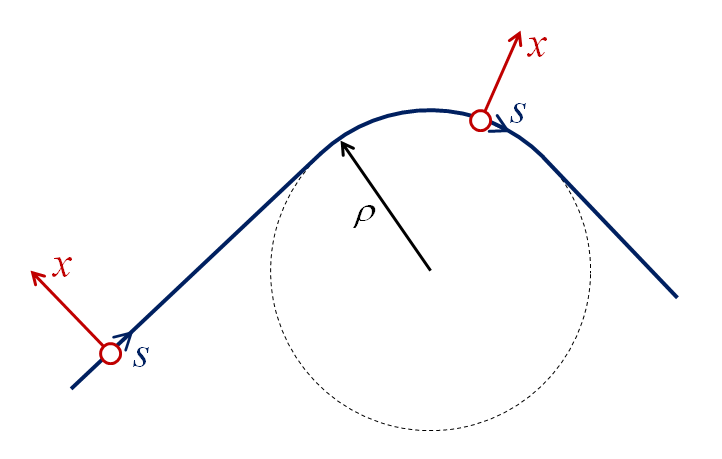
\includegraphics[width=0.8\columnwidth]{ReferenceTrajectory.png}
\caption{Reference trajectory and coordinate system in an accelerator beam line.
The vertical $y$ coordinate is directly out of the page at each location.
\label{fig:referencetrajectory}}
\end{figure}
\end{center}

Particle positions are specified in a \emph{local} cartesian coordinate system.
The distance along the reference trajectory is denoted $s$.  At any point
along the reference trajectory, $x = y = 0$, and the $x$ and $y$ axes are perpendicular
to the local direction of the reference trajectory, and to each other.

The $z$ coordinate is the longitudinal position along the reference trajectory
relative to a particle travelling along the reference trajectory with the
reference momentum.  A positive value for $z$ means that the particle is
\emph{ahead} of the reference particle.

The normalized horizontal canonical momentum is defined by:
\[
p_x = \frac{1}{P_0} \left( \gamma m v_x + qA_x \right),
\]
where $P_0$ is the reference momentum used in specifying the beam rigidity,
$\gamma$ is the relativistic factor corresponding to the particle's velocity,
$m$ is the mass of the particle, $v_x$ is the horizontal component of the
particle's velocity, $q$ is the electric charge on the particle (which should
be the same as used in specifying the beam rigidity), and $A_x$ is the horizontal
component of the vector potential for the magnetic field through which the
particle is moving.  The normalized vertical canonical momentum is defined in
the same way, but with the vertical velocity $v_y$ and vertical component
of the vector potential $A_y$ replacing $v_x$ and $A_x$.

The final dynamical variable, the energy deviation $\delta$, is defined by:
\[
\delta = \frac{E}{P_0 c} - \frac{1}{\beta_0},
\]
where $E$ is the total energy of the particle, $P_0$ is the reference
momentum, $c$ is the speed of light, and $\beta_0$ the speed of a particle
moving with the reference momentum, normalised by the speed of light.

The above definitions for the dynamical variables are used in accelerator
physics because, in most cases, their values remain small as particles move
along a beam line.  This allows some useful approximations to be made when
writing the equations defining how particles move through particular
components.  For ultra-relativistic particles with momenta close to the
reference momentum $P_0$, we can write:
\[
p_x \approx \frac{dx}{ds}, \quad \textrm{and} \quad  p_y \approx \frac{dy}{ds}.
\]
That is, the transverse normalised momenta are approximately equal to the
angle of the particle's trajectory with respect to the reference trajectory.
Also:
\[
\delta \approx \frac{E - E_0}{E_0}
\]
where $E$ is the energy of the particle, and $E_0$ is the reference energy
of the beam.  While these approximations
are useful for visualising the dynamics of a particle, it should be
remembered that they are only approximations valid for small values of the
variables.

Note that if a \texttt{Beam} contains some particles, then the normalised
momenta will automatically be adjusted if the reference momentum (or
reference energy, or beam rigidity) is changed.  The adjustments are made
so that the absolute physical quantities $\gamma m v_x + q A_x$,
$\gamma m v_y + q A_y$, and $E$ remain unchanged if the reference
momentum is change. For example:
\begin{quote}
\texttt{>> beam1 = Beam(Electron); \\
>> GeVdivc = PhysicalUnits.GeV/PhysicalConstants.SpeedOfLight; \\
>> beam1.momentum = 1.0*GeVdivc; \\
>> beam1.particles = [0 0.001 0 0.001 0 0.01]$^\prime$; \\
>> beam1.momentum = 1.1*GeVdivc; \\
>> beam1.particles$^\prime$ \\
ans =    0    0.0009         0    0.0009         0   -0.0818}
\end{quote}

An unusual feature of SAMM compared with other codes is that a \texttt{Beam}
keeps track of the time elapsed since the start of the beam line.  The
elapsed time is stored in the \texttt{globaltime} property of the \texttt{Beam}
class.  This makes it possible for SAMM to determine the electromagnetic
field seen by the beam when it arrives at components with time-dependent
fields (for example, radio-frequency cavities; see Sections~\ref{sec:rfcavity}
and \ref{sec:masteroscillator}).

\subsubsection{Spin\label{subsec:spin}}
As well as tracking the coordinates and momenta of particles along a beam
line, SAMM can track the spins of particles.
Particle spins can be specified in a similar way to the dynamical variables.
The spin of a particle is defined in terms of the orientation of its spin axis with
respect to the reference trajectory in the instantaneous rest frame of the
particle.  For example:
\begin{quote}
\texttt{>> beam1.spins = s;}
\end{quote}
would specify the orientation of the spin of each particle in \texttt{beam1}.
\texttt{s} must be a $2\times N$ matrix, where $N$ is the number of particles
in the beam.  The first row of \texttt{s} gives the polar angle $\theta$ (the
angle of the spin axis of each particle, with respect to the reference trajectory);
the second row of \texttt{s} gives the azimuthal angle $\phi$ (the angle of the
projection of the spin axis on the $x-y$ plane, with respect to the $x$ axis).
Note that $0 \leq \theta \leq \pi$, and $-\pi < \phi \leq \pi$.

For further information, see Section~\ref{sec:spintracking}.


\section{Accelerator components}
Generally, the class definition for an accelerator component will appear
as follows:
\begin{quote}
\begin{verbatim}
classdef AcceleratorComponent < handle
    % AcceleratorComponent class
    
    properties
        length   = 0; % in metres
        aperture = []; % half-axes of elliptical aperture, in metres
    end % properties
    
    methods
    
        function beam = Track(acceleratorcomponent,beam)
            % Apply transfer map for an accelerator component
            
            % Transfer map will be coded here
            
            beam.globaltime = ...
              beam.globaltime + ds/PhysicalConstants.SpeedOfLight;
              
        end % function Track
        
    end % methods
    
end % classdef AcceleratorComponent
\end{verbatim}
\end{quote}

The \texttt{handle} specification in the first line allows different variables to refer to
a single instance of the class: this enables the feature described above,
where the value of a property of all instances of a component in a beam line can be changed
just by changing the value of that property for \emph{any} instance of that component.

Most components will have a number of properties, including (in general): a \texttt{name};
a \texttt{length}; an \texttt{aperture} (see Section~\ref{sec:apertures});
and a number of other properties specific to the type of component (e.g. a field gradient
for a quadrupole magnet).

Every component should have a \texttt{Track} method, that determines the
trajectories of particles through the component.  These are described in more
detail for standard components, in the following sections.  There may be
further methods, depending on the type of component.

%---------------------------------------------------------------------------------------------------

\subsection{Marker}

A marker is a component that has zero length, and has no effect on the beam.
Markers are provided simply as a convenient way to identify particular locations
in a beam line.

\subsubsection{Properties}

\begin{tabular}{|l|l|l|}
\hline
\texttt{name} & & Name of the marker. \\
\texttt{length = 0} & metres & Length of the marker. (Constant) \\
\texttt{aperture = [\,]} & metres & Half-axes of elliptical aperture. (Constant) \\
\hline
\end{tabular}
\vspace{0.2in}

Note that when the aperture is specified as an empty vector [\, ], the component
is treated as having unlimited aperture.

\subsubsection{Methods}

\begin{tabular}{|l|l|}
\hline
\texttt{Track(beam)} & Tracks a beam through the marker. \\
\hline
\end{tabular}
\vspace{0.2in}

%---------------------------------------------------------------------------------------------------

\subsection{Drift space}

A drift space is a field-free section of the beam line.  It has a straight
reference trajectory.

\subsubsection{Properties}

\begin{tabular}{|l|l|l|}
\hline
\texttt{name} & & Name of the drift. \\
\texttt{length} & metres & Length of the drift. \\
\texttt{aperture} & metres & Half-axes of elliptical aperture. \\
\hline
\end{tabular}
\vspace{0.2in}

\subsubsection{Methods}

\begin{tabular}{|l|l|}
\hline
\texttt{Track(beam)} & Tracks a beam through the drift. \\
\hline
\end{tabular}
\vspace{0.2in}

%---------------------------------------------------------------------------------------------------

\subsection{Solenoid}

A field in a solenoid is given by:
\[
B_x = \frac{B_0 g x}{2\left( 1 + g s \right)^2}, \quad
B_y = \frac{B_0 g y}{2\left( 1 + g s \right)^2}, \quad
B_s = \frac{B_0}{1 + g s}.
\]
A solenoid has a straight reference trajectory.  $B_0$ is the field strength
at the entrance of the solenoid, and $g$ (units m$^{-1}$) is a constant
\emph{taper parameter} that characterises a reduction in field strength
along the length of the solenoid.  Note that if $g = 0$, the field is
uniform, and there are no transverse components.

The above components are only an approximation to the field in a tapered
solenoid: although Maxwell's equation $\nabla \cdot \vec{B} = 0$ is exactly
satisfied (for constant $g$), $\nabla \times \vec{B}$ has non-zero transverse
components, implying the existence of either a conduction or a displacement
current.  Usually, there are no currents (apart from the beam current) within
the solenoid.

SAMM includes the fringe fields for a solenoid in the \emph{hard edge}
approximation.  That is, at the entrance to the solenoid, the particles in the
beam receive a kick equivalent to that generated by a field with integrated
components:
\[
\int B_x\, ds = -B_0 x, \quad
\int B_y\, ds = -B_0 y, \quad
\int B_s\, ds = 0,
\]
and similarly at the exit of the solenoid.  However, in an appropriate gauge,
the change in the vector potential on entering the solenoid has the same
magnitude but opposite sign to the change in the mechanical momentum resulting
from the fringe field.  Thus, the change in the \emph{canonical} momentum of
a particle on crossing the fringe field is zero.

\subsubsection{Properties}

\begin{tabular}{|l|l|l|}
\hline
\texttt{name} &   & Name of the solenoid. \\
\texttt{length} & metres       & Length of the solenoid. \\
\texttt{field}  & tesla        & Longitudinal field strength at $s = 0$ ($B_0$). \\
\texttt{taper}  & metre$^{-1}$ & Taper parameter ($g$). \\
\texttt{aperture} & metres & Half-axes of elliptical aperture. \\
\hline
\end{tabular}
\vspace{0.2in}

\subsubsection{Methods}

\begin{tabular}{|l|l|}
\hline
\texttt{Track(beam)}     & Tracks a beam through the solenoid. \\
\texttt{TrackSpin(beam)} & Tracks particle spins through the solenoid. \\
\hline
\end{tabular}
\vspace{0.2in}

%---------------------------------------------------------------------------------------------------

\subsection{Orbit corrector}

An orbit corrector has a dipole field with horizontal and vertical components
(the longitudinal component is zero).  The reference trajectory is a straight line:
therefore, the effect of an orbit corrector will be to deflect a particle initially following
the reference trajectory onto a trajectory at some angle to the reference trajectory.
The deflection angle depends on the field and length of the orbit corrector, and the
charge and momentum of the particle.

\subsubsection{Properties}

\begin{tabular}{|l|l|l|}
\hline
\texttt{name} &   & Name of the orbit corrector. \\
\texttt{length} & metres       & Length of the orbit corrector. \\
\texttt{field}  & tesla        & A two-component vector $[B_x, B_y]$. \\
\texttt{aperture} & metres & Half-axes of elliptical aperture. \\
\hline
\end{tabular}
\vspace{0.2in}

\subsubsection{Methods}

\begin{tabular}{|l|l|}
\hline
\texttt{Track(beam)}     & Tracks a beam through the orbit corrector. \\
\texttt{TrackSpin(beam)} & Tracks particle spins through the orbit corrector. \\
\hline
\end{tabular}
\vspace{0.2in}

%---------------------------------------------------------------------------------------------------

\subsection{Dipole}

A dipole generally has a curved reference trajectory.  In SAMM, the radius of
curvature of the reference trajectory is specified separately from the strength
of the dipole field.  However, in the case that:
\begin{quote}
\texttt{field = rigidity * curvature;}
\end{quote}
a particle travelling with the reference momentum $P_0$ will remain on the
(curved) reference trajectory, if it enters the dipole travelling on the
reference trajectory.

The length of the dipole is the distance along the reference trajectory within
the body of the dipole.

As well as a main field, a field gradient (quadrupole component) can be
specified.  In the case that the field gradient is non-zero, the field on the
reference trajectory will equal the main dipole field: however, this does not
reflect the way that most ``combined function'' dipoles are constructed. 

Fringe fields at the entrance and exit of a dipole have a significant effect
on the dynamics of particles passing through them.  The fringe fields are
specified by the ``pole face rotations'' \texttt{e1} and \texttt{e2} (see
Fig.~\ref{fig:dipolegeometry}), together with the dipole ``aperture'' \texttt{hgap},
and entrance and exit field integrals \texttt{fint1} and \texttt{fint2}.

\begin{center}
\begin{figure}
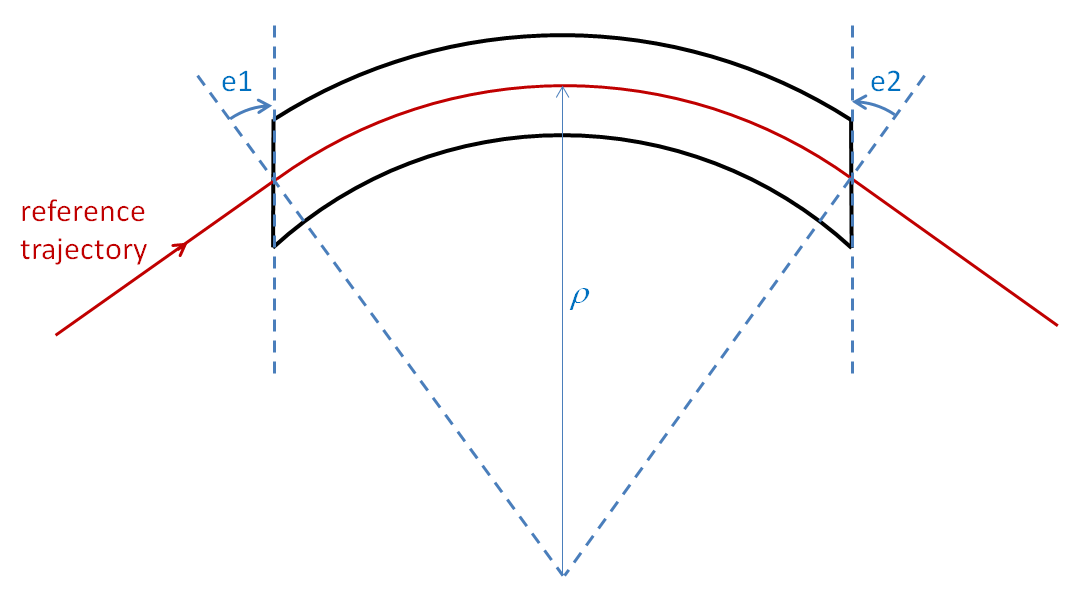
\includegraphics[width=0.8\columnwidth]{DipoleGeometry.png}
\caption{Geometry of a dipole magnet.  If $\texttt{e1} = 0$, then the
entrance face is perpendicular to the reference trajectory; and similarly
if $\texttt{e2} = 0$, then the exit face is perpendicular to the reference trajectory.
\label{fig:dipolegeometry}}
\end{figure}
\end{center}

\subsubsection{Properties}

\begin{tabular}{|l|l|l|}
\hline
\texttt{name} &              & Name of the dipole. \\
\texttt{length}          & metres       & Length.                     \\
\texttt{curvature}       & metre$^{-1}$ & Reciprocal of the radius of curvature \\
                         &              & of the reference trajectory. \\
\texttt{field}           & tesla        & Field strength.             \\
\texttt{gradient}        & tesla/metre  & Strength of quadrupole component. \\
\texttt{hgap}            & metre        & Height of gap between pole faces \\
                         &              & (for calculation of fringe field). \\
\texttt{e1}              & radians      & Rotation angle of entrance face. \\
\texttt{fint1}           &              & Entrance fringe field integral. \\
\texttt{e2}              & radians      & Rotation angle of exit face. \\
\texttt{fint2}           &              & Exit fringe field integral. \\
\texttt{aperture} & metres & Half-axes of elliptical aperture. \\
\hline
\end{tabular}
\vspace{0.2in}

\subsubsection{Methods}

\begin{tabular}{|l|l|}
\hline
\texttt{Track(beam)} & Tracks a beam through the dipole. \\
\texttt{TrackSpin(beam)} & Tracks particle spins through the dipole. \\
\hline
\end{tabular}
\vspace{0.2in}

%---------------------------------------------------------------------------------------------------

\subsection{Quadrupole}
A quadrupole is a magnet in which the strength of the field increases
linearly with distance from the center.  Conventionally, the
\emph{normalised quadrupole gradient} $k_1$ is defined by:
\[
k_1 = \frac{1}{B\rho} \frac{\partial B_y}{\partial x},
\]
where $B\rho$ is the beam rigidity.  Then, in a ``normal'' quadrupole, the field
is given by:
\[
B_x = k_1\,B\rho\,  y, \quad B_y = k_1\,B\rho\, x,  \quad \textrm{and} \quad B_z = 0, 
\]
where $k_1$ is a constant, i.e. $k_1$ is independent of position within the magnet.
(A ``skew'' quadrupole is obtained by rotating a normal quadrupole around the
reference trajectory; skew quadrupoles are not presently implemented in SAMM.)
In SAMM, a quadrupole is specified by its length and the \emph{absolute} gradient
($\partial B_y / \partial x$) in tesla/metre.  SAMM does not use the normalised
gradient.

A particle passing through a quadrupole receives a transverse deflection that
is proportional to the distance of the particle from the reference trajectory:
this results in a focusing (or defocusing) effect on the beam.

\subsubsection{Properties}

\begin{tabular}{|l|l|l|}
\hline
\texttt{name} &              & Name of the quadrupole. \\
\texttt{length}              & metres       & Length.                     \\
\texttt{gradient}            & tesla/metre  & Field gradient. \\
\texttt{aperture} & metres & Half-axes of elliptical aperture. \\
\hline
\end{tabular}
\vspace{0.2in}

\subsubsection{Methods}

\begin{tabular}{|l|l|}
\hline
\texttt{Track(beam)} & Tracks a beam through the quadrupole. \\
\texttt{TrackSpin(beam)} & Tracks particle spins through the quadrupole. \\
\hline
\end{tabular}
\vspace{0.2in}

%---------------------------------------------------------------------------------------------------

\subsection{Sextupole}
A sextupole is a magnet in which the strength of the field increases
nonlinearly with distance from the center.  Conventionally, the
\emph{normalised sextupole gradient} $k_2$ is defined by:
\[
k_2 = \frac{1}{B\rho} \frac{\partial^2 B_y}{\partial x^2},
\]
where $B\rho$ is the beam rigidity.  Then, in a ``normal'' sextupole, the field
is given by:
\[
B_x = k_2\,B\rho\, x y, \quad
B_y = \frac{1}{2} k_2\,B\rho\, (x^2 - y^2),  \quad \textrm{and} \quad
B_z = 0, 
\]
where $k_2$ is a constant, i.e. $k_2$ is independent of position within the magnet.
(A ``skew'' sextupole is obtained by rotating a normal sextupole around the
reference trajectory; skew sextupoles are not presently implemented in SAMM.)
In SAMM, a sextupole is specified by its length and the \emph{absolute} gradient
($\partial^2 B_y / \partial x^2$) in tesla/metre$^2$.  SAMM does not use the normalised
gradient.

Sextupoles are generally used for correcting the variation in focusing strength of
quadrupoles with particle energy (chromaticity).

\subsubsection{Properties}

\begin{tabular}{|l|l|l|}
\hline
\texttt{name} &              & Name of the sextupole \\
\texttt{length}              & metres       & Length.                     \\
\texttt{gradient}            & tesla/metre$^2$  & Field gradient. \\
\texttt{aperture} & metres & Half-axes of elliptical aperture. \\
\hline
\end{tabular}
\vspace{0.2in}

\subsubsection{Methods}

\begin{tabular}{|l|l|}
\hline
\texttt{Track(beam)} & Tracks a beam through the sextupole. \\
\texttt{TrackSpin(beam)} & Tracks particle spins through the sextupole. \\
\hline
\end{tabular}
\vspace{0.2in}

%---------------------------------------------------------------------------------------------------

\subsection{RF cavity\label{sec:rfcavity}}
A radio-frequency (rf) cavity contains an oscillating electromagnetic
field, such that the longitudinal component of the electric field is
given by:
\[
E_z = \frac{V_0}{L} \sin \left( 2\pi f t + \phi \right),
\]
where $V_0$ is the peak voltage across the cavity (in volts), $L$ is the
length of the cavity (in metres), $f$ is the frequency of oscillation
of the field (in hertz), and $\phi$ is the phase angle of the cavity.  $t$
is the time (in seconds), given by the \texttt{globaltime} property of
a \texttt{Beam} object.

Real accelerators generally contain many rf cavities.  To ensure that a
fixed phase relationship is maintained between the different cavities, the
fields are controlled by a common \emph{master oscillator}.  SAMM reflects
this arrangement by providing an abstract class that represents the master
oscillator (Section~\ref{sec:masteroscillator}); the frequency of the
master oscillator is set by a call to the \texttt{SetFrequency} (static)
method of this class.  The frequency of each cavity in a beam line is then
specified as an harmonic of the master oscillator frequency.  The advantage
of this implementation is that the frequencies of all the cavities in a
beam line can be adjusted simultaneously simply by adjusting the
frequency of the master oscillator; the synchronisation between the
different cavities is automatically maintained.

Note that the frequency of the field in an rf cavity can be set in one of
two ways.  If the \texttt{harmonic} property is specified, then the frequency
will be the specified harmonic of the master oscillator frequency (see
Section \ref{sec:masteroscillator}).  If a change is subsequently made to
the master oscillator frequency, the frequency of the cavity is also changed,
so the harmonic relationship is maintained.

Alternatively, the \texttt{frequency} property of the cavity can be set directly.
If this is done, then the frequency of the master oscillator will be changed,
so that the harmonic relationship between the frequency of the cavity and
the master oscillator frequency is maintained.  Note that this will have an
effect on the frequencies of all other cavities in the beam line.

When setting up the rf cavities in a beam line, it is recommended
to set a value for the master oscillator frequency, and then set the
\texttt{harmonic} properties of the cavities.

\subsubsection{Properties}

\begin{tabular}{|l|l|l|}
\hline
\texttt{name} &              & Name of the cavity.         \\
\texttt{length}            & metres       & Length.                             \\
\texttt{voltage}           & volts        & Peak voltage across the cavity.     \\
\texttt{harmonic}          &              & Frequency of the cavity, in units   \\
                           &              & of the master oscillator frequency. \\
\texttt{frequency} & hertz & Frequency of the cavity. \\
\texttt{phase}             & radians      & Phase angle of the cavity.          \\
\texttt{aperture} & metres & Half-axes of elliptical aperture. \\
\hline
\end{tabular}
\vspace{0.2in}

\subsubsection{Methods}

\begin{tabular}{|l|l|}
\hline
\texttt{Track(beam)} & Tracks a beam through the cavity. \\
\hline
\end{tabular}
\vspace{0.2in}

%---------------------------------------------------------------------------------------------------

\subsection{RF accelerating structure\label{sec:rfacceleratingstructure}}
An rf accelerating structure has a same effect on the beam as an rf cavity: the main
difference is that in SAMM, an rf cavity has no effect on the reference momentum,
whereas when the beam passes through an rf accelerating structure, the reference
momentum is changed by an amount corresponding to the change in momentum
of the reference particle.  The values of the dynamical variables of all the particles
in the beam are changed to reflect the change in reference momentum.  For
example, if $P_0$ is the initial reference momentum and $P_1$ is the final reference
momentum, then the transverse momenta $p_x$ and $p_y$ are multiplied by
$P_0/P_1$.

An rf accelerating structure has a number of additional properties compared to an
rf cavity.  The \texttt{structuretype} property should be set to either
\texttt{'StandingWave'} or \texttt{'TravellingWave'}: this will affect the transfer map
used to track particles through the cavity.  For both types of structure, the number of
cells should be specified by setting the \texttt{ncell} property.  In the case of a
standing-wave structure, the total length $L$ should be:
\[
L = n_\mathrm{cell}\frac{c}{2f},
\]
where $n_\mathrm{cell}$ is the number of cells, $f$ the frequency, and $c$ is the
speed of light.

Finally, the \texttt{globalclock} property should be set to \texttt{true} or \texttt{false}
(the default is \texttt{true}).  In general, each particle in the beam will see an electric
field in the rf accelerating structure given by:
\[
E_z = \frac{V_0}{L} \cos \! \left( 2\pi f t + \phi_0 \right),
\]
where $V_0$ is the \texttt{voltage} of the structure; $L$ is the \texttt{length}; $f$
is the \texttt{frequency}; and $\phi_0$ is the \texttt{phase}.  If the \texttt{globalclock}
property is set to \texttt{true}, then the phase of the cavity is locked to the global clock,
so that $t = T - z/c$, where $T$ is the time elapsed on the global clock (the time taken
for the reference particle to move along the beam line to the accelerating structure)
and $z$ is a dynamical variable (the longitudinal co-ordinate of the particle).
If the \texttt{globalclock} property is set to \texttt{false}, then $t = -z/c$, i.e. the
time elapsed on the global clock is ignored.

The properties \texttt{harmonic} and \texttt{frequency} can be set in the same way,
and have the same effect, as the corresponding properties for an rf cavity
(Section \ref{sec:rfcavity}).

\subsubsection{Properties}

\begin{tabular}{|l|l|l|}
\hline
\texttt{name} &              & Name of the accelerating structure.         \\
\texttt{structuretype}            &   & Type of structure: \texttt{'TravellingWave'} or \texttt{'StandingWave'}.      \\
\texttt{length}            & metres       & Length.                             \\
\texttt{ncell}            &        & Number of cells in the structure.                             \\
\texttt{voltage}           & volts        & Peak voltage across the structure.     \\
\texttt{harmonic}          &              & Frequency of the structure, in units   \\
                           &              & of the master oscillator frequency. \\
\texttt{frequency} & hertz & Frequency of the structure. \\
\texttt{phase}             & radians      & Phase angle of the structure.          \\
\texttt{globalclock}             &    & Flag (true or false) to set synchronisation.          \\
\texttt{aperture} & metres & Half-axes of elliptical aperture. \\
\hline
\end{tabular}
\vspace{0.2in}

\subsubsection{Methods}

\begin{tabular}{|l|l|}
\hline
\texttt{Track(beam)} & Tracks a beam through the cavity. \\
\hline
\end{tabular}
\vspace{0.2in}

%---------------------------------------------------------------------------------------------------

\subsection{Master oscillator\label{sec:masteroscillator}}
A master oscillator cannot be included as a component in a beam line.  The
\texttt{MasterOscillator} class in SAMM is declared as an \emph{abstract class},
which means it is not possible to define an object of that type.  However,
the \texttt{MasterOscillator} class has a method \texttt{SetFrequency} that
is declared as \emph{static}: thus the \texttt{SetFrequency} method can be called
to define the value of the global variable \texttt{MasterOscillatorFrequency}
without creating an instance of the class.  That is, the command:
\begin{quote}
\texttt{>> MasterOscillator.SetFrequency(500e6);}
\end{quote}
without any preceding definitions, will set the value of 
\texttt{MasterOscillatorFrequency} to 500\,MHz.

To see the value of \texttt{MasterOscillatorFrequency} in the Matlab workspace,
issue the command:
\begin{quote}
\texttt{>> global MasterOscillatorFrequency}
\end{quote}

%---------------------------------------------------------------------------------------------------

\subsection{Beam position monitor}
A beam position monitor (BPM) simply records the mean values of the $x$ and $y$
coordinates of all the particles in a \texttt{Beam} as the beam passes through
the BPM.  It makes no changes to the values of the dynamical variables for the
particles.  The mean values of the transverse coordinates are stored in a
\texttt{buffer} (a property of the \texttt{BeamPositonMonitor} class), which is
an array of limited size.  Each time a \texttt{Beam} passes through a BPM, the
mean coordinates are recorded in the next ``column'' of the \texttt{buffer}; once
the end of the \texttt{buffer} array is reached, new values are recorded starting
again from the beginning of the \texttt{buffer} array, with new values being
overwritten.

\subsubsection{Properties}

\begin{tabular}{|l|l|}
\hline
\texttt{type = 'beampositionmonitor'} & Component type.  (Constant)   \\
\texttt{length = 0}        & Length.  (Constant)           \\
\texttt{bufferpointer}     & Column of \texttt{buffer} array where next \\
                           & position values will be recorded. (Private) \\
\texttt{buffer}            & $2\times b$ array of recorded mean $x$ and $y$ \\
                           & particle coordinates, where $b$ is the buffer size. \\
\hline
\end{tabular}
\vspace{0.2in}

\subsubsection{Methods}

\begin{tabular}{|l|l|}
\hline
\texttt{Track(beam)} & Tracks a beam through the BPM. \\
\texttt{ResetBuffer(buffersize)} & Clears buffer and resets to size \texttt{buffersize}. \\
\hline
\end{tabular}
\vspace{0.2in}


\section{Accelerator physics}

\subsection{Particle tracking}
Tracking particles through components is achieved by applying transfer maps
that relate values of the dynamical variables at the exit of the element
to the values at the entrance to the element.  For example, the
transfer map for a drift of length $L$ may be represented
(in the ultra-relativistic limit, $\gamma \to \infty$) as:
\begin{eqnarray*}
x_1      & = & x_0 + \frac{p_{x0} L}{\sqrt{(1+\delta_0)^2 - p_{x0}^2 - p_{y0}^2}}, \\
p_{x1}   & = & p_{x0}, \\
y_1      & = & y_0 + \frac{p_{y0} L}{\sqrt{(1+\delta_0)^2 - p_{x0}^2 - p_{y0}^2}}, \\
p_{y1}   & = & p_{y0}, \\
z_1      & = & z_0 + \left( 1 - \frac{1+\delta_0}{\sqrt{(1+\delta_0)^2 - p_{x0}^2 - p_{y0}^2}} \right) L, \\
\delta_1 & = & \delta_0,
\end{eqnarray*}
where a subscript ``0'' denotes the value of the dynamical variable at the
start of the drift, and the subscript ``1'' denotes the value of the variable
at the exit of the drift.

As described in Section~\ref{sec:modellingabeam}, particle positions are specified
in a local cartesian coordinate system. At any point along the reference
trajectory, $x = y = 0$, and the $x$ and $y$ axes are perpendicular to the
local direction of the reference trajectory, and to each other (see
Fig.~\ref{fig:referencetrajectory}).  The $z$ coordinate is the longitudinal position
along the reference trajectory relative to a particle travelling along the reference
trajectory with the reference momentum.  A positive value for $z$ means that the
particle is \emph{ahead} of the reference particle.

The normalized horizontal canonical momentum is defined by:
\[
p_x = \frac{1}{P_0} \left( \gamma m v_x + qA_x \right),
\]
where $P_0$ is the reference momentum used in specifying the beam rigidity,
$\gamma$ is the relativistic factor corresponding to the particle's velocity,
$m$ is the mass of the particle, $v_x$ is the horizontal component of the
particle's velocity, $q$ is the electric charge on the particle (which should
be the same as used in specifying the beam rigidity), and $A_x$ is the horizontal
component of the vector potential for the magnetic field through which the
particle is moving.  The normalized vertical canonical momentum is defined in
the same way, but with the vertical velocity $v_y$ and vertical component
of the vector potential $A_y$ replacing $v_x$ and $A_x$.

The energy deviation $\delta$ is defined by:
\[
\delta = \frac{E}{P_0 c} - \frac{1}{\beta_0},
\]
where $E$ is the total energy of the particle, $P_0$ is the reference
momentum, $c$ is the speed of light, and $\beta_0$ the speed of a particle
moving with the reference momentum, normalised by the speed of light.

With the above definitions, the variables $(x,p_x)$, $(y,p_y)$ and
$(z,\delta)$ form three sets of \emph{canonical conjugate pairs}; that is,
the equations of motion may be expressed as Hamilton's equations:
\[
\frac{dx}{ds} = \frac{\partial H}{\partial p_x}, \qquad
\frac{dp_x}{ds} = -\frac{\partial H}{\partial x},
\]
and similarly for $(y,p_y)$ and $(z,\delta)$.  The function
$H = H(x,p_x,y,p_y,z,\delta ;s)$ is the Hamiltonian, which defines
the dynamics of the system.  For the present application, the
Hamiltonian may be written as:
\begin{eqnarray}
H = -(1 + hx)\sqrt{\left( \frac{1}{\beta_0} + \delta - \frac{q\phi}{P_0c} \right)^2 - (p_x - a_x)^2 - (p_y - a_y)^2 - \frac{1}{\beta_0^2 \gamma_0^2}} \nonumber \\
 - (1 + hx)a_s + \frac{\delta}{\beta_0}, \nonumber
\end{eqnarray}
where $h=1/\rho$ is the curvature of the reference trajectory, $P_0$ is
the reference momentum, $q$ the electric charge on the particle, $\beta_0$
and $\gamma_0$ the relativistic velocity and relativistic factor (respectively),
and the components of the normalised vector potential are given by:
\[
a_x = \frac{q}{P_0}A_x, \quad a_y = \frac{q}{P_0}A_y, \quad \textrm{and} \quad
a_s = \frac{q}{P_0}A_s.
\]
In general, the transfer map for any component is obtained by:
\begin{enumerate}
\item writing down the scalar and vector potentials for the electromagnetic
fields in the component;
\item constructing the Hamiltonian using the expressions for the scalar
and vector potentials;
\item integrating Hamilton's equations over the length of the component.
\end{enumerate}
Exact solutions to Hamilton's equations can be written in closed algebraic
form only for very simple accelerator components; in general, some
approximations need to be made.

In SAMM, the transfer map for a given component is encoded in the
\texttt{Track} method of the corresponding class.  The \texttt{Track} method
takes a \texttt{Beam} as a parameter, and applies the transfer map to each
particle in the \texttt{Beam}; the \texttt{Track} method then returns the new
values of the dynamical variables for all the particles.

The \texttt{Beamline} class also has a \texttt{Track} method; this simply
passes a \texttt{Beam} to the \texttt{Track} method for each of the components
over a specified range of the \texttt{Beamline} in turn.

\subsection{Transfer matrices}
For small changes in the intial values of the dynamical variables, it is often
possible to approximate the changes in the final values over a section of
beam line by a linear map, that is:
\[
\Delta \vec{x}(s_1) = \mathbf{M}(s_1,s_0;\vec{x}(s_0)) \cdot \Delta \vec{x}(s_0),
\]
where: $\Delta \vec{x}(s_0)$ is a vector representing small changes in the values
of the dynamical variables at a location $s_0$ on the reference trajectory;
$\mathbf{M}(s_1,s_0;\vec{x}(s_0))$ is a matrix with elements that are determined by the
parameters of the accelerator components between locations $s_0$ and $s_1$ on
the reference trajectory; and $\Delta \vec{x}(s_1)$ is a vector representing
small changes in the dynamical variables at a location $s_1$, resulting from
the small changes $\Delta \vec{x}(s_0)$.  The matrix $\mathbf{M}(s_1,s_0;\vec{x}(s_0))$
is known as the \emph{transfer matrix} from $s_0$ to $s_1$, about the
trajectory defined by the initial values of the dynamical variables $\vec{x}(s_0)$.

Transfer matrices can be computed in SAMM using the \texttt{ComputeTransferMatrix}
function.  For example:
\begin{quote}
\texttt{>> m = ComputeTransferMatrix(bl,[n1 n2],rigidity,[0 0 0 0 0 0]');}
\end{quote}
will compute the transfer matrices from the entrance of component \texttt{n1} in
the beam line \texttt{bl}, to the exit of each component up to component \texttt{n2}
(where \texttt{n1} and \texttt{n2} are integers), assuming beam rigidity given by \texttt{rigidity} (in units of tesla-metres), and trajectory starting on the
reference trajectory.  The result \texttt{m} is a three-dimensional array, in which
\texttt{m(:,:,n)} is a $6\times 6$ matrix representing the transfer matrix
from the entrance of the first component in the range to the entrance of
the $n^\textrm{th}$ component in the range (so that \texttt{m(:,:,1)} is the
identity matrix).

\subsection{Closed orbits and dispersion}
If the beam in a storage ring is stable, then there must exist a trajectory
that repeats (closes on) itself exactly after one turn around the storage ring.
This trajectory is known as the \emph{closed orbit}.  Generally, in designing
a storage ring, the reference trajectory is designed to close on itself after
one turn.  However, errors (for example, in dipole strength or the frequencies
of rf cavities) usually mean that the reference trajectory is not a physical
trajectory for a particle in the accelerator.  The problem then is to compute
the closed orbit (with respect to the reference trajectory) with given
components with specified parameters.

Closed orbits can be computed in SAMM using the \texttt{ComputeClosedOrbit}
function.  For example:
\begin{quote}
\texttt{>> [closedorbit m] = ComputeClosedOrbit(bl,beam);}
\end{quote}
will return in \texttt{closedorbit} a $6\times (N+1)$ matrix giving the
values of the dynamical variables along the closed orbit at the exit/entrance
of each component, where there are $N$ components in the beam line, for a
\texttt{beam} object of class \texttt{Beam}.  Each row of $m$
corresponds to a dynamical variable; the first column corresponds to the
entrance of the beam line, and the last column represents the exit (for a
closed storage ring, these points are the same).  The $6\times 6$ matrix
$m$ contains the transfer matrix about the closed orbit for one complete
turn around the storage ring, starting at the entrance of the beam line.

In a storage ring, the closed orbit followed by a particle depends on the
energy of the particle.  The change in closed orbit with respect to the
energy deviation is called the \emph{dispersion}:
\[
\eta_x = \frac{dx_\textrm{\tiny co}}{d\delta}, \qquad
\eta_{px} = \frac{dp_{x,\textrm{\tiny co}}}{d\delta},
\]
where the subscript ``co'' indicates the value of the dynamical variable
on the closed orbit.
SAMM does not compute the dispersion directly.  However, the energy of
particles on the closed orbit can be changed by changing the frequency
of the master oscillator\footnote{The usual way of measuring the dispersion
in a real storage ring is by changing the frequency of the rf cavities,
and measuring the resulting change in beam position using the BPMs.  It
is worth thinking through how this works}.  Therefore, by computing
the closed orbit in SAMM with small changes to the frequency of the
master oscillator, the dispersion can easily be found.

\subsection{Lattice functions}
Lattice functions are used to describe the linear optics of a beam line.
For example, if the horizontal motion is independent of the vertical and
longitudinal motion, and the closed orbit coincides with the reference
trajectory, then the distribution in horizontal phase space (that is,
a plot of $p_x$ \emph{vs} $x$) of particles in a beam is given by:
\begin{eqnarray*}
\langle x^2 \rangle   & = &  \beta_x \varepsilon_x, \\
\langle xp_x \rangle  & = & -\alpha_x \varepsilon_x, \\
\langle p_x^2 \rangle & = &  \gamma_x \varepsilon_x,
\end{eqnarray*}
where the brackets $\langle\, \rangle$ indicate an average over all particles
in the beam, the lattice functions $\beta_x$, $\alpha_x$ and $\gamma_x$ are functions
of the position along the reference trajectory, and the \emph{horizontal
emittance} $\varepsilon_x$, is constant as the beam moves along a beam line
consisting of linear components (i.e. components for which the transfer map
is linear in the dynamical variables).  The lattice functions, also called the
\emph{Twiss parameters}, are defined so that they satisfy the condition:
\[
\beta_x \gamma_x - \alpha_x^2 = 1,
\]
from which it follows that:
\[
\varepsilon_x = \sqrt{\langle x^2 \rangle \langle p_x^2 \rangle - \langle xp_x \rangle^2}.
\]

In a storage ring, one can in principle inject a bunch of particles with any
distribution at some point in the ring; then, in general, after one complete turn,
the distribution will have changed.  However, there will be a unique distribution
that remains unchanged after one turn.  The Twiss parameters describing this
distribution are said to be \emph{matched} to the storage ring.

Lattice functions are used routinely in the analysis of accelerator beam
lines, and are extremely useful for describing a range of properties of a
given beam line.  In SAMM, the matched lattice functions in a storage ring can
be computed using the function \texttt{ComputeMatchedTwiss}.  For example:
\begin{quote}
\texttt{>> [beta tune closedorbit] = ComputeMatchedTwiss(bl,beam);}
\end{quote}
will return the lattice functions in the 4--dimensional array \texttt{beta}, the
phase advances (see below) in the array \texttt{tune}, and the closed
orbit in the array \texttt{closedorbit}.  \texttt{bl} is the beam line for the
complete storage ring, and \texttt{beam} is an object of class \texttt{Beam}.

In general, there will be coupling between the degrees of freedom, so that the
horizontal motion depends on the vertical and the longitudinal, the vertical
depends on the horizontal and longitudinal, and the longitudinal motion depends
on the horizontal and vertical.  However, it is possible always to define
three invariant quantities, the \emph{beam emittances} $\varepsilon_\textrm{\tiny I}$,
$\varepsilon_\textrm{\tiny II}$, and $\varepsilon_\textrm{\tiny III}$, that describe the
``volume'' of the bunch in phase space.  The beam distribution at any point along
the beam line is then given by:
\[
\langle x_i x_j \rangle = \sum_{k=\textrm{\tiny I},\textrm{\tiny II},\textrm{\tiny III}}
\beta_{ij}^k \varepsilon_k,
\]
where $x_i$ is the $i^\textrm{th}$ dynamical variable, and $\beta_{ij}^k$ generalise
the horizontal Twiss parameters $\beta_x$, $\alpha_x$ and $\gamma_x$ to three
degrees of freedom.  For example, in the limit of weak coupling, we have
$\beta_x = \beta_{11}^\textrm{\tiny I}$, and $\alpha_x =-\beta_{12}^\textrm{\tiny I}$.
The 4--dimensional array \texttt{beta} returned by
\texttt{ComputeMatchedTwiss} is indexed so that \texttt{beta(i,j,k,n)} gives the
value of the lattice function $\beta_{ij}^k$ at the entrance of the $n^\textrm{th}$
component in the beam line.

As particles move along a beam line, their motion can be represented in terms of
simple harmonic motion, with amplitude and frequency that varies with position
along the beam line.  For example, for uncoupled horizontal motion, and again assuming
that the closed orbit coincides with the reference trajectory, we can write:
\begin{eqnarray*}
x(s) & = & \sqrt{2\beta_x J_x(s)} \cos \left( \phi_x(s) \right), \\
p_x(s) & = & -\sqrt{\frac{2J_x(s)}{\beta_x}} \left[ \sin \left( \phi_x(s) \right)  + 
                                           \alpha_x \cos \left( \phi_x(s) \right) \right].
\end{eqnarray*}
In this form, we represent the motion of a particle as it moves along the beam
line, as an oscillation around the reference trajectory.
The variables $(\phi_x,J_x)$, known as \emph{action-angle variables}, form
a canonically conjugate coordinate and momentum pair of dynamical variables that
can be used as an alternative to the pair $(x,p_x)$.  In a linear approximation
to the motion in the electromagnetic fields of accelerator components, the action $J_x$
is constant, and the angle $\phi_x$ increases monotonically.  In three degrees of
freedom, there are three action and three angle variables; the change in each of
the three angle variables from the start of the beam line to the exit of each
component along the beam line is given by the $3\times (N+1)$ array \texttt{tune},
returned by a call to the function \texttt{ComputeMatchedTwiss}.  The total phase
advance around a storage ring divided by $2\pi$ is called the \emph{tune} of the
storage ring: the tune is the total number of oscillations made by the particle
around the reference trajectory (or, more generally, the closed orbit) in one
complete turn around the ring.  Transverse oscillations are known as \emph{betatron}
oscillations, and longitudinal oscillations are known as \emph{synchrotron}
oscillations.

\subsection{Synchrotron radiation integrals}
Relativistic charged particles in an accelerator emit electromagnetic radiation,
known as synchrotron radiation, as they move through electric and magnetic
fields.  The effect of the radiation on the motion of the particles is
strongest for electrons moving through dipole magnets: in most other cases,
(nearly always for proton or ion beams; and almost always for electrons
moving in quadrupoles, rf cavities, etc.) the radiation effects are weak
enough to be ignored.

In an electron storage ring, synchrotron radiation leads to the beam
achieving an equilibrium distribution, corresponding to the matched lattice
functions and particular values for the three beam emittances, after
a sufficient number of turns.  The strength of the radiation effects,
and the equilibrium beam emittances, are characterised by a set of
\emph{synchrotron radiation integrals}.  Assuming that the closed orbit
coincides with the reference trajectory, these are defined in a planar
storage ring by:
\begin{eqnarray*}
I_1 & = & \int \frac{\eta_x}{\rho} \, ds, \\
I_2 & = & \int \frac{1}{\rho^2} \, ds, \\
I_3 & = & \int \frac{1}{\left| \rho^3 \right|} \, ds, \\
I_4 & = & \int \frac{\eta_x}{\rho} \left( \frac{1}{\rho^2} + 2k_1 \right) \, ds, \\
I_5 & = & \int \frac{\mathcal{H}}{\left| \rho^3 \right|} \, ds.
\end{eqnarray*}
Here, $\rho$ is the local radius of curvature of the reference trajectory;
$\eta_x$ is the dispersion; $k_1$ is the normalised quadrupole gradient.
For calculating the equilibrium beam sizes in a storage ring, the integrals
should be taken over the entire ring, but the integrals can, in principle, be
computed over any section of any beam line.

The function $\mathcal{H}$ appearing in the fifth radiation integral is
given in terms of the dispersion and Twiss parameters:
\[
\mathcal{H} = \gamma_x \eta_x^2 + 2 \alpha_x \eta_x \eta_{px} + \beta_x \eta_{px}^2.
\]

In SAMM, the synchrotron radiation integrals can be computed by a call
to the function \texttt{ComputeRadiationIntegrals}.  For example:
\begin{quote}
\texttt{>> [I1 I2 I3 I4 I5] = ComputeRadiationIntegrals(bl,beam);}
\end{quote}
\texttt{bl} is a beam line, and \texttt{beam} is an object of class \texttt{Beam}.  The
values of the radiation integrals, over the complete beam line (assumed to be
a complete storage ring) are returned in \texttt{I1}, \texttt{I2}, \texttt{I3},
\texttt{I4}, and \texttt{I5}.

\subsection{Spin tracking\label{sec:spintracking}}
SAMM evolves the spin vector $\vec{S}$ a particle through the field of a component
using the Thomas-BMT equation \cite{cite:koutchouk}:
\[
\frac{d\vec{S}}{dt} = \vec{\Omega} \times \vec{S},
\]
where:
\[
\vec{\Omega} = -\frac{q}{\gamma m} \left[
( 1 + G\gamma)\vec{B}_\perp + (1 + G)\vec{B}_\parallel -
\left( G + \frac{1}{1+ \gamma} \right) \gamma \beta \times
\frac{\vec{E}}{c}
\right] ,
\]
$q$ is the charge of a particle, $m$ the mass of a particle, $\gamma$
the relativistic factor, $\beta$ the speed of the particle divided by
the speed of light, $\vec{B}_\perp$ is the component of the magnetic field
perpendicular to the velocity of the particle, $\vec{B}_\parallel$ is the
component of the magnetic field parallel to the velocity of the particle,
and $\vec{E}$ is the electric field.  $G$ is the gyromagnetic anomaly for the
particle, given by:
\[
G = \frac{g-2}{2},
\]
where $g$ (simply called the $g$-factor) gives the magnetic moment of the particle:
\[
\vec{\mu} = \frac{g}{2} \frac{e\hbar}{2m} \hat{S},
\] 
where $\hat{S}$ is a unit vector in the direction of the spin axis.  In the
Dirac theory for point-like, spin-$\frac{1}{2}$ charged particles, $g = 2$;
quantum field theory leads to small corrections to this value
($g \approx 2.002319$ for positrons), which are measured by $G$.

In an accelerator, the magnetic fields are usually large compared to the
magnitudes of the electric fields (divided by the speed of light).  SAMM
neglects the effects of any electric fields (e.g. from RF cavities) on the
spins of particles in the beam.

\section{Examples}
SAMM is distributed with a number of examples, including:

\paragraph{\texttt{DemoTracking}} demonstrates tracking particles multiple times
through a beam line to produce phase space plots for the horizontal,
vertical and longitudinal motion.

\paragraph{\texttt{DemoBeamlineAnalysis}} demonstrates computation of the closed
orbit, lattice functions and synchrotron radiation integrals.

\paragraph{\texttt{DemoSpinTracking}} demonstrates tracking the spin of a particle
through a solenoid.
\vspace{0.2in}

All of these examples are scripts that can be invoked directly from
the Matlab command line:
\begin{quote}
\texttt{>> DemoStorageRingAnalysis \\
>> DemoBunchTracking \\
>> DemoChromaticity}
\end{quote}

\texttt{DemoTracking} and \texttt{DemoBeamlineAnalysis} each calls
\texttt{DefineBeamline} (another script) that defines the beam line used in
each case.

\section{Some useful references}

There are many good books on accelerator physics.  The difficulty is that
there is a variety of different notations, conventions, and approaches used
for the subject.  However, the basic concepts of accelerator components
(including dipoles, quadrupoles, rf cavities, BPMs etc.) and beam dynamics
(including closed orbit, dispersion, lattice functions, synchrotron
radiation) are all widely discussed.

A good introduction is provided by the proceedings of the CERN Accelerator
Schools, e.g. \cite{cite:CAS1994}.

The books by Lee \cite{cite:lee}, Wiedemann \cite{cite:wiedemann} and
Edwards and Syphers \cite{cite:edwardssyphers} provide useful introductions.

The particular approach taken by SAMM to particle tracking is described in
more detail in a set of lecture notes \cite{cite:wolski1, cite:wolski2}.
There are many different approaches taken towards coupling; the formalism
used in SAMM is described in \cite{cite:wolski3}.

\begin{thebibliography}{99}

\bibitem{cite:matlab}
Mathworks, \texttt{http://www.mathworks.co.uk/}

\bibitem{cite:matlabdoc}
\texttt{http://www.mathworks.co.uk/access/helpdesk/help/techdoc/}

\bibitem{cite:mad8}
Methodical Accelerator Design (MAD), \\
\texttt{http://mad.web.cern.ch/mad/}

\bibitem{cite:koutchouk}
See, for example:
J.\,Buon and J.\,P.\,Koutchouk, ``Polarization of Electron and Proton Beams,''
CERN Accelerator School, 5th Advanced Accelerator Physics Course,
Rhodes, Greece (20 September--1 October, 1993), CERN 95-06. \\
\texttt{http://cdsweb.cern.ch/record/254747/files/CERN-95-06.pdf}

\bibitem{cite:CAS1994}
CERN Accelerator School, 5th General Accelerator Physics Course,
Jyv\"askyl\"a, Finland (7--18 September, 1992), CERN-94-01. \\
\texttt{http://documents.cern.ch/cgi-bin/ \\
setlink?base=cernrep\&categ=Yellow\_Report\&id=94-01\_v1} \\
\texttt{http://documents.cern.ch/cgi-bin/ \\
setlink?base=cernrep\&categ=Yellow\_Report\&id=94-01\_v2} \\
See in particular the articles by Rossbach and Schm\"user, Wilson,
and Le Duff.

\bibitem{cite:lee}
S.Y.\,Lee, ``Accelerator Physics,'' World Scientific, 2nd edition (2005).

\bibitem{cite:wiedemann}
H.\,Wiedemann, ``Particle Accelerator Physics,'' Springer, 3rd edition (2007).

\bibitem{cite:edwardssyphers}
D.A.\,Edwards and M.J.\,Syphers, ``An Introduction to the Physics
of High Energy Particle Accelerators,'' Wiley (1993).

\bibitem{cite:wolski1}
A.\,Wolski, ``Linear Dynamics in Particle Accelerators,''
Cockcroft Institute Lecture Course (2007). \\
\texttt{http://pcwww.liv.ac.uk/$\sim$awolski/main\_teaching\_lineardynamics.htm}

\bibitem{cite:wolski2}
A.\,Wolski, ``Nonlinear Dynamics in Particle Accelerators,''
Cockcroft Institute Lecture Course (2009). \\
\texttt{http://pcwww.liv.ac.uk/$\sim$awolski/main\_teaching\_nonlineardynamics.htm}

\bibitem{cite:wolski3}
A.\,Wolski, ``Alternative Approach to General Coupled Linear Optics,''
Phys.\,Rev.\,ST\,Accel.\,Beams 9, 024001 (2006).

\end{thebibliography}

\end{document}